% DRAFT, rewrite
\section{Architectural design}

\subsection{Overview}
The app keeps its four layers: views, observable models, the store layer and the
platform. The update adds no layer. It extends the store layer so that a load is
made of parts, and it adds a row of policies: small value types with no state of
their own that decide order, deadlines, budget, prefetch and changes. Policies take
the clock and the device state as arguments, so each is tested without a network,
a phone or waiting.

\begin{figure}[H]
\centering
\begin{tikzpicture}[
  band/.style={draw, rounded corners=3pt, text width=14.6cm, align=left, inner sep=6pt, font=\small},
  uses/.style={-{Stealth[length=5pt]}, thin}]
  \newcommand\comp[1]{\fbox{\strut #1}\hspace{3pt}}
  \node[band] (ui) {\textbf{Views}\\[3pt]
    \comp{Screens} \comp{Section kit: \texttt{arriving}, RevealRenderer, SectionStatus, ShapeMemory}};
  \node[band, below=0.45cm of ui] (models) {\textbf{Observable models} (main actor)\\[3pt]
    \comp{Query} \comp{FreeRoomsModel} \comp{CampusMapModel} \comp{SearchModel} \comp{NewMarks} \comp{BoundaryClock}};
  \node[band, below=0.45cm of models] (policies) {\textbf{Policies} (pure values, new)\\[3pt]
    \comp{RelevanceOrder} \comp{DeadlinePolicy} \comp{SpeculativeBudget} \comp{TimetablePrefetch} \comp{ChangeDetector}};
  \node[band, below=0.45cm of policies] (store) {\textbf{Store layer} (actors)\\[3pt]
    \comp{Resource} \comp{Progress} \comp{Loader} \comp{PartStore} \comp{RequestGate} \comp{LoadingLedger} \comp{OfflinePack}};
  \node[band, below=0.45cm of store] (platform) {\textbf{Platform and existing services}\\[3pt]
    \comp{HTTP} \comp{OfflineStore} \comp{BackgroundRefresh} \comp{FreshnessCoordinator} \comp{NetworkMonitor} \comp{DevicePressure} \comp{NotificationModel} \comp{UpdateFeed} \comp{DiagnosticsReport}};
  \draw[uses] (ui) -- (models);
  \draw[uses] (models) -- (policies);
  \draw[uses] (policies) -- (store);
  \draw[uses] (store) -- (platform);
\end{tikzpicture}
\caption{Components by layer. An arrow means ``uses''; a layer also uses every layer below it.}
\end{figure}

\subsection{Component view}
New components are marked (new); the others exist and change.

\begin{description}[style=nextline, leftmargin=1.5em]
  \item[Resource] Declares one kind of remote data. Gains an optional \texttt{Part} type and a max age per part. A resource with one request declares nothing and compiles unchanged.
  \item[Progress (new)] The typed handle a fetch reports parts through. Replaces the untyped task-local \texttt{Partial.sink}. Holds only the newest snapshot not yet consumed.
  \item[Loader] One actor per resource. Now keeps an entry per part, asks the resource only for the parts that are missing or too old, files each part when it arrives, and applies the DeadlinePolicy.
  \item[PartStore (new)] Reads and writes one file per part and account on top of \texttt{OfflineStore}, with the fetch time. Written atomically.
  \item[Query] The observable handle a view reads. Gains which parts have arrived, which failed, where each came from (stored copy or network), and the changes of the last refresh.
  \item[RequestGate (new)] One actor for all hosts. Admits requests in two lanes, on-screen and speculative, caps speculative requests per host, tracks timeouts per host and fails fast while a host is not responding. Reports every request to the ledger.
  \item[LoadingLedger (new)] An actor that appends one small entry per request and per screen opening to a capped file, and computes the report.
  \item[RelevanceOrder (new)] Orders the rooms of a campus from the map area on screen, the next lecture's building and the favourite campus.
  \item[DeadlinePolicy (new)] Says, for a part and the time it has been waiting, whether to keep waiting or to show the stored copy.
  \item[SpeculativeBudget (new)] Says whether a speculative request may be sent now, from the network path, the device pressure, the student's settings and today's count.
  \item[TimetablePrefetch (new)] From the timetable and the current time, lists the parts to warm.
  \item[OfflinePack (new)] Owns the list of parts of the pack, runs it in a processing task, and publishes what is stored and how old.
  \item[BoundaryClock (new)] Computes the next booking boundary from stored bookings and wakes the models that show rooms.
  \item[ChangeDetector (new)] Compares the items of a fetched part with its stored copy by identity and returns what was added, changed and removed.
  \item[NewMarks (new)] Keeps, per account, the identities of items marked as new until their section has been on screen.
  \item[Section kit (new)] The shared interface pieces: the \texttt{arriving} modifier, RevealRenderer, SectionStatus and ShapeMemory.
  \item[Existing services] \texttt{BackgroundRefresh} gains the prefetch call and a processing task. \texttt{FreshnessCoordinator} calls the prefetch after a pass. \texttt{UpdateFeed} becomes one consumer of ChangeDetector. \texttt{DiagnosticsReport} gains the ledger section.
\end{description}

\subsection{Deployment view}
Everything runs on the student's iPhone. There is no server of the project.

\begin{center}\small
\begin{tabularx}{\linewidth}{@{}l X@{}}
  \toprule
  Node & What runs or lives there \\
  \midrule
  App process, foreground & All components. Requests run in both lanes. \\
  App process, refresh task & Agenda and career refresh as today, then TimetablePrefetch, within 30 seconds. \\
  App process, processing task & OfflinePack only. May be stopped by iOS at any time; resumes from PartStore. \\
  Widget extension & Reads the shared container, as today. Sends no request. \\
  App group container & PartStore files, NewMarks, the offline pack's state, the ledger file. \\
  Keychain & Tokens, as today. Never read by the new components. \\
  Politecnico's hosts & Answer HTTPS requests. Unchanged. \\
  \bottomrule
\end{tabularx}
\end{center}

\subsection{Component interfaces}
The signatures fix names and responsibilities; bodies and access levels are decided
in the code.

\begin{lstlisting}
// Resource: parts are optional. Part == Whole means "one request".
protocol Resource: Sendable {
    associatedtype Part: Hashable & Sendable & CaseIterable = Whole
    static func maxAge(of part: Part) -> TimeInterval        // default: ttl
    func fetch(_ key: Key, env: Env, parts: Set<Part>,
               over held: Value?, progress: Progress<Self>) async throws -> Value
}

struct Progress<R: Resource>: Sendable {
    func report(_ value: R.Value, arrived: Set<R.Part>, failed: Set<R.Part> = [])
}

actor Loader<R: Resource> {
    func value(_ key: R.Key, env: Env, force: Bool,
               progress: Progress<R>?) async throws -> Snapshot
    func warm(_ keys: some Sequence<R.Key>, env: Env)        // speculative lane
    func clear()                                             // sign-out
}

struct PartStore: Sendable {
    func save<V: Codable>(_ value: V, part: String, of name: String, account: String)
    func load<V: Codable>(_ type: V.Type, part: String, of name: String,
                          account: String) async -> (value: V, age: TimeInterval)?
    func removeAll(account: String)
}

@MainActor @Observable final class Query<R: Resource> {
    var value: R.Value? { get }
    func phase(of part: R.Part) -> LoadPhase
    func has(_ parts: R.Part...) -> Bool
    var changes: ChangeSet { get }                            // last refresh
}

enum LoadPhase: Equatable {
    case held(age: TimeInterval), waiting(since: Duration), arrived, empty
    case failed(String)
}

actor RequestGate {
    enum Lane { case onScreen, speculative }
    func run<T: Sendable>(host: String, lane: Lane, part: String,
                          _ request: @Sendable () async throws -> T) async throws -> T
    func isOpen(_ host: String) -> Bool                       // false while failing fast
}

actor LoadingLedger {
    func record(_ entry: RequestEntry)
    func opened(_ screen: String) -> ScreenToken
    func firstContent(_ token: ScreenToken)
    func completed(_ token: ScreenToken)
    func used(_ speculative: RequestID)
    func report(days: Int) async -> LedgerReport
    func erase()
}
\end{lstlisting}

\begin{lstlisting}
// Policies: values in, decision out. No clock, no singletons.
enum RelevanceOrder {
    static func order(_ rooms: [Classroom], visible: Set<BuildingID>,
                      nextLecture: BuildingID?, favourite: CampusID?) -> [Classroom]
}
struct DeadlinePolicy {
    var deadline: Duration = .seconds(4)
    func decision(waited: Duration, hasStoredCopy: Bool) -> Decision  // .wait | .showStored
}
struct SpeculativeBudget {
    struct Device { var lowData, metered, lowPower: Bool; var thermal: ThermalLevel }
    struct Settings { var allowMetered: Bool; var dailyLimit: Int = 600 }
    func allows(_ count: Int, device: Device, settings: Settings, sentToday: Int) -> Int
}
enum TimetablePrefetch {
    static func wanted(now: Date, lectures: [AgendaEvent],
                       lead: TimeInterval = 3600) -> [PrefetchItem]
}
enum ChangeDetector {
    static func changes<I: Identifiable & Equatable>(from old: [I], to new: [I]) -> ChangeSet
}
\end{lstlisting}

\begin{lstlisting}
// Section kit.
extension View {
    func arriving(_ phase: LoadPhase, title: LocalizedStringKey,
                  retry: (() async -> Void)? = nil) -> some View
    func revealed(order: Int, isNew: Bool) -> some View
    func screenLedger(_ name: String) -> some View
}
\end{lstlisting}

\subsection{Runtime view}

\subsubsection{UC1: a screen built from several parts}
\begin{figure}[H]
\centering
\begin{tikzpicture}
  \lifeline{v}{0}{View}
  \lifeline{q}{3.2}{Query}
  \lifeline{l}{6.4}{Loader}
  \lifeline{r}{9.6}{Resource}
  \lifeline{s}{12.8}{PartStore}
  \msg{0}{3.2}{1.2}{load()}
  \msg{3.2}{6.4}{1.8}{value(key, progress)}
  \msg{6.4}{12.8}{2.4}{load stored parts}
  \msg{6.4}{9.6}{3.0}{fetch(missing parts)}
  \msg[dashed]{9.6}{6.4}{3.9}{report(part A)}
  \msg{6.4}{12.8}{4.5}{save(part A)}
  \msg[dashed]{6.4}{3.2}{5.1}{snapshot, arrived \{A\}}
  \msg[dashed]{3.2}{0}{5.7}{phase(A) = arrived}
  \msg[dashed]{9.6}{6.4}{6.6}{report(part B) \dots}
  \msg[dashed]{6.4}{3.2}{7.2}{final value}
  \msg[dashed]{3.2}{0}{7.8}{all parts arrived}
\end{tikzpicture}
\caption{A load with parts. Each request inside \texttt{fetch} passes through RequestGate, which records it in the ledger.}
\end{figure}

The loader passes the resource only the parts that have no stored copy younger
than their max age (\idref{R15}, \idref{R16}). Reports are buffered newest-only and
the query consumes them at most every 100 ms (\idref{R4}). If the view goes away,
the fetch is cancelled as today, and the parts already saved stay (\idref{R14}).
When a part has waited longer than the deadline and a stored copy exists, the
loader hands the query that copy with \texttt{held(age:)} and keeps the request
running (\idref{R17}).

\subsubsection{UC2: free rooms}
\begin{enumerate}
  \item FreeRoomsModel asks RelevanceOrder for the order of the campus's rooms, giving it the buildings on the map, the next lecture's building and the favourite campus.
  \item It requests bookings eight at a time in that order through the occupancy loader, on the on-screen lane.
  \item After each batch it assigns the rooms received so far; the list and the map observe them.
  \item BoundaryClock computes the earliest booking boundary among the stored bookings and sleeps until then.
  \item At the boundary the model recomputes ``free now'' from stored bookings, and requests again the rooms on screen, once (\idref{R24}, \idref{R25}).
\end{enumerate}

\subsubsection{UC3: prefetch before a lecture}
\begin{figure}[H]
\centering
\begin{tikzpicture}
  \renewcommand\seqdepth{6.6}
  \lifeline{t}{0}{Trigger}
  \lifeline{p}{3.4}{TimetablePrefetch}
  \lifeline{b}{6.8}{SpeculativeBudget}
  \lifeline{l}{10.0}{Loaders}
  \lifeline{g}{13.0}{RequestGate}
  \msg{0}{3.4}{1.2}{wanted(now, lectures)}
  \msg[dashed]{3.4}{0}{1.8}{items}
  \msg{0}{6.8}{2.6}{allows(count, device, settings)}
  \msg[dashed]{6.8}{0}{3.2}{granted n}
  \msg{0}{10.0}{4.0}{warm(first n keys)}
  \msg{10.0}{13.0}{4.6}{run(host, speculative)}
  \msg[dashed]{13.0}{10.0}{5.4}{answer}
\end{tikzpicture}
\caption{Prefetch. RequestGate records each request in the ledger. The trigger is FreshnessCoordinator after a foreground pass, or BackgroundRefresh.}
\end{figure}

When the student later opens the room or the course, the loader finds the part
fresh and sends nothing (\idref{R20}); the ledger marks the speculative request as
used (\idref{R36}).

\subsubsection{UC4: no connection}
\begin{enumerate}
  \item The query asks the loader; the loader restores every stored part from PartStore.
  \item NetworkMonitor reports no connection, so RequestGate fails requests at once.
  \item Parts with a stored copy are \texttt{held(age:)}; parts without are \texttt{failed}; the section kit shows each accordingly (\idref{R23}).
  \item When the connection returns, FreshnessCoordinator runs a pass and only parts older than their max age are requested.
\end{enumerate}

\subsubsection{UC5: a change}
\begin{enumerate}
  \item A refresh brings a part that has a stored copy.
  \item Before filing it, the loader hands old and new items to ChangeDetector.
  \item The change set goes to the query (\texttt{changes}), to NewMarks, and to UpdateFeed, whose existing policy decides whether to notify (\idref{R29}).
  \item The section kit reveals only items in the change set and shows the mark; when the section has been on screen, NewMarks removes them (\idref{R27}, \idref{R28}).
\end{enumerate}

\subsubsection{UC6: the ledger}
\texttt{screenLedger} opens a token when a screen appears, the first \texttt{arriving}
section to reach \texttt{arrived} or \texttt{held} marks first content, and the
last marks completion. DiagnosticsReport asks the ledger for the report over 14
days.

\subsection{Selected architectural styles and patterns}
\begin{itemize}
  \item \textbf{Layers}, as today: a view never talks to a loader, a loader never to a view.
  \item \textbf{Functional core, imperative shell}: decisions live in policies that are pure; actors and models only carry them out.
  \item \textbf{Actors for coordination}: Loader, RequestGate and LoadingLedger hold shared state; work proportional to a payload stays in \texttt{@concurrent} functions.
  \item \textbf{Observer} through Observation: models are \texttt{@Observable} on the main actor.
  \item \textbf{Stale-while-revalidate}, now per part.
  \item \textbf{Circuit breaker} per host, inside RequestGate.
\end{itemize}

\subsection{Other design decisions}
\begin{description}[style=nextline, leftmargin=1.5em]
  \item[1. Progress is a parameter, not a task-local.] Alternative: keep \texttt{Partial.sink}. A task-local cannot be generic, so it is untyped and cast back, and it cannot say which parts arrived. Cost: the \texttt{fetch} signature changes; a default implementation forwards to the old one for resources without parts.
  \item[2. One file per part.] Alternative: one file per resource, rewritten when each part arrives. Per-part files make each write small and atomic, so a kill between two parts loses nothing (\idref{R14}, \idref{R16}), and each carries its own age (\idref{R15}). Cost: restoring reads several small files; \idref{P5} bounds it.
  \item[3. A deadline shows the stored copy and keeps the request.] Alternatives: cancel and retry, or send a second request in parallel. Both add load on the Politecnico's hosts, against assumption D11, and a late answer is still the freshest data.
  \item[4. The breaker is per host, in one gate.] Alternative: per resource. A timeout says something about the host, and all resources on that host benefit at once (\idref{R18}). One gate is also the only place that sees every request, which the ledger and the lanes need.
  \item[5. Prefetch follows the timetable, not habits.] Relies on assumption D5. A learned predictor needs data the ledger does not have yet and is out of scope.
  \item[6. Changes are found by identity, generically.] Alternative: one detector per kind of data, as UpdateFeed does today for exams. Relies on assumption D10. Values expose their items as \texttt{Identifiable \& Equatable}; kinds without stable ids are not compared.
  \item[7. The ledger is the app's own file.] Alternatives: signposts or MetricKit alone. Signposts cannot be read back on the phone, and MetricKit delivers one aggregate a day without per-part detail. The ledger stores no content (\idref{R38}).
  \item[8. A boundary is one sleep until a known instant.] Relies on assumption D6. It is not polling: nothing is sent unless a boundary passed and the screen is visible.
  \item[9. The offline pack uses a processing task.] The refresh task's 30 seconds cannot hold it (assumption D7). The pack is resumable because every part is filed when it arrives.
  \item[10. No separate package yet.] The store layer stays in the app target until this update has shipped; \texttt{Packages/} is also ignored by git today. Moving it is a later, mechanical step.
\end{description}
